% !TEX TS-program = xelatex
% !TEX encoding = UTF-8 Unicode

% GSET Summer 2021 - Tennessee Technological University
% Tristan Hill - June 04, 2021
% Rocket Deisgn Challenge - Initial Brainstorm

\documentclass[12pt]{article}

% Custom Preamble
\usepackage{/home/thill/Documents/lectures/cpp_workshop/modules/cpp_tutorial} 

% Title and Misc
\newcommand{\MNUM}{0} %Module Number
\newcommand{\MNAME}{Introduction to C++} %Module Name
\newcommand{\TNAME}{Brainstorm} %Tutorial Name
\pagestyle{myheadings}
\markright{{\large GSET - Programming with Mr. Hill}}

\begin{document}

\thispagestyle{plain}

\begin{center}
   {\bf \large GSET - Programming with Mr. Hill - Summer 2021} \vspace{5mm}\\
   {\bf \Large \MNAME \hspc -  Rocket Design Challenge - \TNAME}\vspace{3mm}\\
   
\end{center}

 \hspace*{3cm}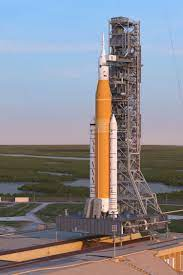
\includegraphics[scale=.6]{rocket_launch.jpeg} \hspace*{1cm}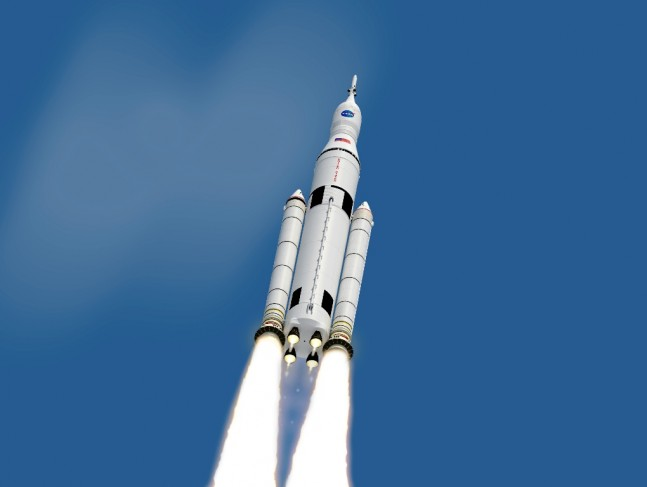
\includegraphics[scale=.28]{Space-Launch.jpg}


\begin{description}[labelindent=1cm]
	
	\item[\textbf{\underline{Mission Overview:}}] \hfill \vspace{3mm}\\
	The goal is to send a rocket into space and collect as data about the flight of the rocket and the environmental conditions throughout the flight. There are many design aspects required for this mission to be successful.
	
		\begin{itemize}
			\item {\bf Fuselage Design:} The rocket will be constructed of materials available at TNTech.
			\item {\bf Propulsion and Control Design:} The rocket should fly as high as possible in a controlled manner.
			\item {\bf Electronics Design:} Useful data regarding the rocket flight and environment should be collected for post flight analysis.
			\item {\bf Measurement and Data Analysis Design:} The data collection and analysis should be relevant to the mission.
		\end{itemize}
	
\newpage		
	\item[\textbf{\underline{Available Hardware:}}] \hfill \vspace{0mm}
	A prototype of the rocket must be completed in time to launch and analyze the acquired data. The following hardware is available for experimentation and use in the prototype rocket. 

\begin{itemize}
	\item {\bf Propulsion:} Estes c-65, solid fuel rocket  engines and ignitors.
	\item {\bf Fuselage:} Various 3D printing plastics, various laser cutting materials, traditional machining materials
	\item {\bf Electronics:}
		\begin{itemize}
			\item On-board Computer: 
				\begin{enumerate}
					\item Arduino Nano328p 
					 \hspace*{2cm}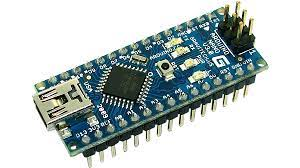
\includegraphics[scale=.3]{arduino_nano.jpeg}
					 \hspace*{0.5cm}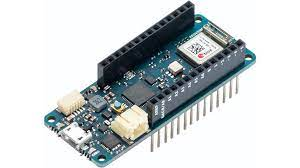
\includegraphics[scale=.3]{arduino_mkr.jpeg}
					\item Arduino MKR1010wifi
				\end{enumerate}
			\item Flight Data Measurement System:
				\begin{itemize}
					\item BNO055 Absolute Orientation Sensor 
					\hspace*{0.5cm}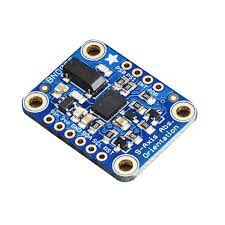
\includegraphics[scale=.3]{bno_055.jpeg}
					\hspace*{0.5cm}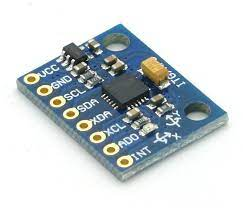
\includegraphics[scale=.3]{gy521.jpeg}
					\item GY-521 (ITG/MPU)
				\end{itemize}
			\item Environment Data Measurement System:
			\begin{itemize}
				\item DPS310 Temperature and Barometric Pressure Sensor 
				\hspace*{0.5cm}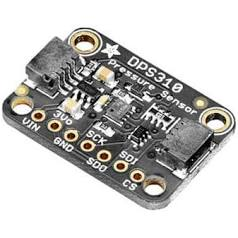
\includegraphics[scale=.3]{dps310.jpeg}
				\hspace*{0.5cm}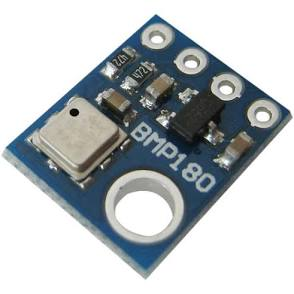
\includegraphics[scale=.3]{gy68.jpeg}
				\item GY-68 (BMP180) Barometric Pressure, Temperature and Altitude Sensor
			\end{itemize}
			\item Data Storage System:
				\begin{itemize}
					\item 5v Ready SD Card Breakout Board
					\hspace*{0.5cm}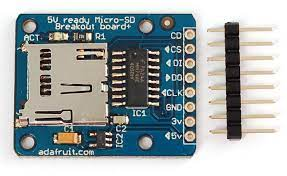
\includegraphics[scale=.3]{sdcard_reader.jpeg}
					\hspace*{0.5cm}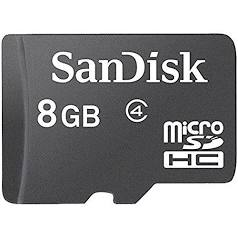
\includegraphics[scale=.3]{sd_card.jpeg}
					\item 8G or 16G micro SD card (SDHC) 
					
				\end{itemize}
			
		\end{itemize}
\end{itemize}


\newpage

\item[\textbf{\underline{Part 1 - Initial Brainstorm:}}] \hfill \vspace{0mm}


	Generate initial ideas about the mission as a group and document the promising design ideas.






\end{description}
\end{document}

